\documentclass[journal]{IEEEtran}

\usepackage{lipsum}
\usepackage{siunitx}
\usepackage{tikz}
\usepackage[american]{circuitikz}
\usepackage{colortbl}
\usepackage{amsmath}

\graphicspath{{Figs/}}


\hyphenation{op-tical net-works semi-conduc-tor}


\begin{document}
\title{Low Power Digital Beamforming\\ with Approximate Compute for Mobile Ultrasound Systems}

% author names and IEEE memberships
% note positions of commas and nonbreaking spaces ( ~ ) LaTeX will not break
% a structure at a ~ so this keeps an author's name from being broken across
% two lines.
% use \thanks{} to gain access to the first footnote area
% a separate \thanks must be used for each paragraph as LaTeX2e's \thanks
% was not built to handle multiple paragraphs
%

\author{Josh~Kay, Karthik~Gopalan % <-this % stops a space
\thanks{Karthik Gopalan and Josh Kay are graduate student researchers at the University of California, Berkeley.}}% <-this % stops a space




% make the title area
\maketitle

% As a general rule, do not put math, special symbols or citations
% in the abstract or keywords.
\begin{abstract}
As the size of 2D transducer arrays for ultrasound systems increase, the hardware complexity, die area, and power of digital beamforming circuits increases by the number of elements squared; moreover, as ultrasonic imaging systems trend toward mobile applications, modern beamforming techniques do not address the growing power and area restrictions demanded by these applications. Approximate computing (AC) introduces a technique to reduce power and area in integrated digital circuits. By implementing an adaptive minimum variance (MV) beamformer with approximate compute arithmetic blocks, lower power and area will be achieved while mitigating image resolution loss compared to conventional delay-and-sum beamformers. An adaptive minimum variance beamformer implemented with approximate compute provides adequate image resolution while minimizing power and area to be beneficial toward mobile ultrasound applications. 
\end{abstract}

\begin{IEEEkeywords}
Beamforming, Transducer, Approximate Computing, Minimum Variance, Delay-and-Sum.
\end{IEEEkeywords}


\IEEEpeerreviewmaketitle



\section{Introduction}

\IEEEPARstart{H}{igh} frequency ultrasound imaging is an effective tool for medical diagnosis due to its non-invasive, real time body imaging capability. Evolution of ultrasonic imaging technology from single element transducers to 2D transducer arrays improved focusing techniques for both the transmitting and receiving operations of the ultrasonic imaging device \cite{2dCMUT}. Receive focusing is known as beamforming and may be implemented with a series of delays and adders. However, the growing number of elements in 2D ultrasonic imaging devices have greatly increased the rate at which data needs to be transmitted from the system front-end and processed by the beamformer. Additionally, the increase in transmission and processing rates have greatly increased circuit area and power consumption in traditional digital beamformers \cite{ultrasoundLinearArray}. These shortcomings become increasingly more prevalent as ultrasonic imaging devices transition to mobile platforms \cite{mobileUltrasound}. 



Approximate computing (AC) has recently emerged as a promising technique for reducing power and area in digital integrated circuits. The principle behind AC is using deterministic hardware that will produce low order errors but can be built with much fewer resources. For example, adder cells can be designed with only 10 transistors by utilizing XOR/XNOR gates and pass transistor style muxes \cite{yang2013approximate}. The use of pass transistors in these adders reduces the noise margin and can therefore produce less accurate results compared to a conventional CMOS adder which uses 28 transistors. Han et. al implemented an inverse discrete cosine transform algorithm with approximate adders and simulated a 38\% energy savings compared to an exact computation \cite{han2013approximate}.

Beamforming implemented with approximate compute offers an attractive solution for mobile ultrasound systems that require low power, small area and only moderate accuracy. This project explores the use of approximate compute techniques for beamforming implementations in mobile ultrasound applications. 

\section{Problem Description}

\subsection{Area and Power Limitations in Beamforming}

Advances in ultrasonic imaging system technology have enabled larger transducer arrays, resulting in greater control of delay and weighting of each array element for receive beamforming. Beamforming enables dynamic scan depth focusing as opposed to fixed focal lengths of single element transducer systems \cite{Szabo}. However, more elements in transducer arrays inherently produce beamforming architectures that suffer from increased area and power dissipation. This increase in power and area is compounded by the desire for higher resolution images that demand higher transmission and image processing rates. A push toward mobile applications has put increasing pressure on ultrasonic imaging systems to be low power while occupying smaller area. Therefore, emerging beamforming techniques must maintain high quality imaging while minimizing power dissipation and area. 

Modern beamforming techniques attempt to remedy the tradeoffs between power and resolution and between area and resolution through various techniques. Wagner reduced power dissipation by reducing processing rates in a technique describe as compressed beamforming. In compressed beamforming, low power is achieved by beamforming the sub-Nyquist samples obtained from multiple transducer elements; however, increased beamformer complexity translated to greater area when implemented on chip \cite{Wagner}. Feldkamper proposed a low power iterative algorithm for calculating delay information for each channel in a beamforming configuration. The design consisted of only 8 adders and 8 registers per channel but limits the image resolution \cite{feldkamper2000low}. In \cite{gurun2012analog}, an analog dynamic delay-and-sum beamformer was proposed for high frequency ultrasonic imagers. The method used a current-mode first-order all-pass filter topology with an enhancement technique on the current mirrors to increase the bandwidth. Although this method dissipated relatively low power for higher frequency systems, the analog beamformer required considerably more area. 

The increased complexity of ultrasonic systems coupled with a growing trend in mobile ultrasonic applications creates a need for low power, small area beamforming with adequate accuracy. Although prior works demonstrate beamforming techniques that manipulate these tradeoffs, an optimal beamforming solution for mobile ultrasound applications has not been explored. 

\subsection{Approximate Compute Tradeoffs}
When designing with approximate computing techniques the main trade off is between accuracy and power. A designer must consider how much accuracy can be compromised before the result of the computation is unusable. Another metric that is not often considered is the NRE cost due to the lack of tool support for designing inexact circuits. Adders and multipliers provided in most PDKs must be replaced with hand tuned approximate configurations. Despite these challenges, many groups have successfully implemented numerous algorithms with low precision hardware. For instance, one group was able to implement a 560 \si{\nano\watt} heartbeat detection and classification circuit by using variable precision approximate compute adders \cite{amirtharajah2004micropower}.

When applied to beamforming in mobile ultrasonic applications, the inaccuracies introduced by AC must not mitigate the resolution improvements due to beamforming. In other words, AC beamforming integration must provided enough resolution improvement to justify the increased power and area caused by the added beamformer hardware. 

\section{Solution}

In this work, a method for beamforming is proposed using approximate compute arithmetic blocks. Implementing beamforming with AC inherently reduces power and area at the expense of accuracy; however, the reduced resolution of a beamforming solution with AC may be suitable for mobile applications. Therefore, the goal of this work is to identify if AC beamforming integration presents an acceptable solution for ultrasonic mobile applications.

\begin{figure}
    \centering
    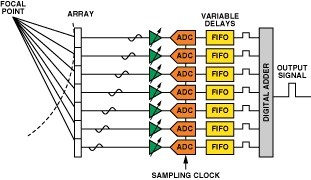
\includegraphics[width=0.4\textwidth]{beamform.jpg}
    \caption{Block Diagram of typical Digital Beamformer}
    \label{fig:beamform}
\end{figure}

Delay-and-sum (DAS) beamforming is a conventional technique in medical ultrasound imaging. Depicted in figure \ref{fig:beamform}, this technique delays a received signal by array elements appropriate to the distances from the main target of the imaging and then sums the delayed signals to construct the echo signal originating from the main target. Although this technique for beamforming is common in medical ultrasound systems due to its simplicity, DAS is a non-adaptive beamforming. Consequently, DAS beamformed signals have large side lobes, resulting in low resolution and weak suppression of interfering signals. Therefore, traditional DAS beamformers will not be suitable for an AC beamformer implementation due to the expected degradation in resolution from AC inaccuracies. To combat the expected errors from the approximate compute arithmetic blocks, an adaptive minimum variance (MV) beamforming technique will be implemented. The improved resolution from MV beamforming will forgive some of the inaccuracies due to AC \cite{synnevag2007adaptive}.  

A set of full adder cells that employ approximate computing techniques will be designed. These include but are not limited to an accurate XNOR based adder with pass transistors, a 6 transistor XOR adder that is accurate for 4 of 8 inputs, and an 8 transistor XOR based adder that is accurate for 6 out of 8 inputs. These full adder cells will be used in ripple-carry adders, carry-lookahead adders, and multipliers.

We hope that the use of approximate computing will result in the power savings necessary for modern digital beamforming. For low precision applications with a low energy budget, the authors expect that approximate computing is a viable option.

\section{Experiment}

The purpose of this project is to determine if adaptive minimum variance beamforming implemented with approximate compute is a viable option for mobile ultrasound applications. To determine this, two MV beamformer will be designed in the 28nm/32nm technology: one design implemented with AC arithmetic blocks and one design implemented with conventional arithmetic blocks. The following approximate compute arithmetic blocks will be implemented: the 8T XOR adder, the 6T XNOR adder, and the 8T XNOR adder. The MV beamformer will be designed in a modular fashion such that arithmetic blocks can be interchanged for easy comparison. The power, area, and image resolution of each implementation will be anaylzed.

\subsection{Adaptive Minimum Variance Beamforming}

The method for adpative MV beamforming is described in \cite{synnevag2007adaptive}. An transducer is assumed to contain an array of M, where each element records a signal $x_m(t)$. $P+1$ scatterers will be considered with each scatterer with a reflected signal $s_p(t)$. $s_0(t)$ describes the signal that originated from the focal point of the receiver. Under these assumptions, equation \ref{eq:time_delay} describes the $m$th time-delayed channel.

    \begin{equation}\label{eq:time_delay}
    x_m(t) = \frac{1}{r_{m,0}} \, s_0(t) + \sum_{p=1}^{P} \, \frac{1}{r_{m,p}} \, s_p(t) * \delta(t - \tau_{m,p}) + n_m(t)
   \end{equation}
   
   In equation \ref{eq:time_delay}, $r_{m,p}$ is the distance from the reflected object $p$ to the receiver sensor $m$, $\delta(t)$ is the Dirac delta-function, $\tau_{m,p}$ is the delay from the reflected object $p$ to the receiver sensor $m$, $n_m(t)$ is the noise on channel $m$, and ($*$) is the convolution operator. The $M$ observed time-delays are then ordered in a vector, $\textbf{X}(t)$. With each channel delayed to focus at a point in the image, the adaptive beamformer computes the the optimal aperature shading before combining the channels. The weighted sum output of the spatial measurements is described by: 
   
    \begin{equation}\label{eq:weighted_output}
    z(t) = \sum_{m=0}^{M-1} \, w_m(t)x_m(t) = \textbf{w}(t)^H \, \textbf{X}(t)
   \end{equation}

    where $w_m(t)$ is the aperature weight for the sensor $m$ and $\textbf{w}(t) = [w_0(t) w_1(t) .. w_{M-1}(t)]^H$. The MV achieves minimum variance (power) of $z(t)$ while maintaining unit gain in the focal point. This is achieved by applying the following weights to equation \ref{eq:weighted_output}:  
    
    \begin{equation}\label{eq:weights}
    \textbf{w}(t) = \frac{\textbf{R}(t)^{-1} \, \textbf{a}}{\textbf{a}^H \, \textbf{R}(t)^{-1} \, \textbf{a}}
   \end{equation}
   
   where $\textbf{R}(t)$ is the spatial covariance matrix and $\textbf{a}$ is a vector of ones.

\subsection{10T Accurate XNOR Adder}
\begin{figure}
\centering
\begin{circuitikz}[scale=0.6]
    \draw (0,0)
        node[nmos] (a1) {}
        ++(3,0) node[nmos] (b1) {}
        ($(a1.D)!0.5!(b1.D)$) ++(0,3) node[pmos] (a2) {} 
        ++(0,3) node[pmos] (b2) {}
        (b1) ++(3,0) node[nmos] (in1) {}
        ++(3,0) node[nmos] (in2) {}
        ($(in1.D)!0.5!(in2.D)$) ++(0,3) node[pmos] (ip1) {} 
        ++(0,3) node[pmos] (cin2) {}
        ($(in1.D)!0.5!(in2.D)$) ++(0,-4) node[pmos, rotate = 90] (cin1) {} 
        ++(0,-3.5) node[nmos,rotate = 270] (a3) {} 
    ;
    
    \draw
        (a1.G) node[left] {A}
        (b1.G) node[left] {B}
        (a2.G) node[left] {A}
        (b2.G) node[left] {B}
        (a3.S) node[left] {A}
        (cin2.G) node[left] {$C_{in}$}
        (cin1.S) -- ++(-0.5,0) node[left] {$C_{in}$}
        ($(a3.D)!0.5!(cin1.D)$) -- ++(2,0) node[right] {$C_{out}$}
        (in2.D) -- ++(2,0) node[right] {Sum}
        (in1.S) -| (in2.G)
        (cin1.S) -| (in1.S)
        (in1.D) -- (in2.D)
        ($(in1.D)!0.5!(in2.D)$) -- (ip1.D)
        (ip1.S) -- (cin2.D)
        (ip1.G) node[left] {I}
        (in2.S) node[below] {I}
        (in1.G) node[left] {I}
    ;    
        
    \draw
        (a1.S) node[below] {B}
        (b1.S) node[below] {A}
        (a2.S) -- (b2.D)
        (b2.S) ++(-0.5,0) -- ++(1,0) ++(-0.5,0) node[above] {$V_{DD}$}
        (cin2.S) ++(-0.5,0) -- ++(1,0) ++(-0.5,0) node[above] {$V_{DD}$}
        (a1.D) -- (b1.D)
        ($(a1.D)!0.5!(b1.D)$) -- (a2.D)
        (cin1.G) -- (a3.G)
        (a3.D) -- (cin1.D)
        (b1.D) -- ++(1,0) node[right] {I}
    ;
\end{circuitikz}
\caption{10T Accurate XNOR Adder}
\label{fig:XA1}
\end{figure}

We will design the accurate XNOR based adder shown in figure \ref{fig:XA1}. The gates will be sized in order to minimize average delay across all inputs. The circuit uses two XNOR gates and a set of pass transistors. The node I is internal to the circuit and labelled for clarity. The reader should note that no transistor is tied to the lower supply, therefore the lower noise margins are expected to be worse than the upper noise margins. Verification of the functionality of the circuit is left as an exercise to the reader.

\subsection{8T Approximate XOR Adder}
\begin{figure}
\centering
\begin{circuitikz}[scale=0.6]
    \draw (0,0)
        node[nmos,rotate=270] (cin1) {}
        (cin1.D) ++(6,-1) node[nmos] (gnd1) {}
        ++(0,2) node[pmos] (vdd1) {}
        (cin1.G) ++(3.5,0) node[pmos] (coutb1) {}
        (coutb1.S) ++(-2,2.5) node[nmos,rotate=270] (in1) {}
        ++(0,3.5) node[pmos,rotate=90] (ip1) {}
        ($(in1)!0.5!(ip1)$) ++(4,-1) node[nmos,xscale=-1] (gnd2) {}
        ++(0,2) node[pmos,xscale=-1] (vdd2) {}
    ;
    \draw
        (gnd1.S) node[ground] {}
        (cin1.S) node[left] {$C_{in}$}
        (vdd1.S) ++(-0.5,0) -- ++(1,0) ++(-0.5,0) node[above] {$V_{DD}$}
        (gnd2.S) node[ground] {}
        (vdd2.S) ++(-0.5,0) -- ++(1,0) ++(-0.5,0) node[above] {$V_{DD}$}
    ;
    \draw  
        (gnd1.D) -- (vdd1.D)
        ($(gnd1.D)!0.5!(vdd1.D)$) -- ++(1,0) node[right] {$C_{out}$}
        (gnd1.G) -- (vdd1.G)
        (gnd2.G) -- (vdd2.G)
        ($(gnd1.G)!0.5!(vdd1.G)$) -| (cin1.D)
        (coutb1.G) -- (cin1.G)
        (cin1.D) -| (coutb1.D)
        (in1.D) -| (coutb1.S)
        (in1.S) -| (cin1.G)
        (ip1.S) -| (cin1.G)
        (in1.G) -- (ip1.G)
        ($(in1.G)!0.5!(ip1.G)$) -- ++(1,0) node[right] {B}
        (ip1.D) -- ++(0,2) -- ++(5,0) -| ($(gnd2.G)!0.5!(vdd2.G)+(1,0)$)
        ($(gnd2.G)!0.5!(vdd2.G)$) -- +(1,0) node[right] {A}
        ($(gnd2.D)!0.5!(vdd2.D)$) -| ($(in1.D)+(0.7,0)$)
        (cin1.S) ++(0.5,0) -- ++(0,-1) node[below] {Sum}
    ;
\end{circuitikz}
\caption{8T Approximate XOR Adder (AXA1)}
\label{fig:AXA1}
\end{figure}

The 8 transistor approximate XOR based adder is shown in figure \ref{fig:AXA1}. The outputs that the circuit generates are shown in the equations below:
\begin{align*}
    Sum &= C_{in} \\
    C_{out} &= \overline{(A \oplus B)C_{in} + \bar{A}\bar{B}}
\end{align*}

The carry output is regenerative while the Sum output will adopt the noise of the input $C_{in}$. The truth table for this adder cell is shown in table \ref{tab:AXA1_Truth} where the incorrect outputs are highlighted in red. The adder cell will be designed by sizing gates for minimum average delay across all possible inputs. 

\begin{table}
    \centering
    \begin{tabular}{c c c | c | c}
         A & B & $C_{in}$ & $C_{out}$ & Sum \\ \hline
         0 & 0 & 0 & 0 & 0 \\ 
         0 & 0 & 1 & 0 & 1 \\ 
         0 & 1 & 0 & \cellcolor{red!25}1 & \cellcolor{red!25}0 \\ 
         0 & 1 & 1 & \cellcolor{red!25}0 & \cellcolor{red!25}1 \\ 
         1 & 0 & 0 & \cellcolor{red!25}1 & \cellcolor{red!25}0 \\ 
         1 & 0 & 1 & \cellcolor{red!25}0 & \cellcolor{red!25}1 \\ 
         1 & 1 & 0 & 1 & 0 \\ 
         1 & 1 & 1 & 1 & 1 \\ 
    \end{tabular}
    
    \caption{Truth Table for AXA1}
    \label{tab:AXA1_Truth}
\end{table}

\subsection{6T Approximate XNOR Adder}
\begin{figure}
\centering
\begin{circuitikz}[scale=0.6]
    \draw (0,0)
        node[nmos] (a1) {}
        ++(3,0) node[nmos] (b1) {}
        ($(a1.D)!0.5!(b1.D)$) ++(0,3) node[pmos] (a2) {} 
        ++(0,3) node[pmos] (b2) {}
        ($(a1.D)!0.5!(b1.D)$) ++(4.5,-1.75) node[nmos,rotate = 270] (a3) {}
        ($(a1.D)!0.5!(b1.D)$) ++(4.5,1.75) node[pmos, rotate = 90] (cin1) {}
    ;
    
    \draw
        (a1.G) node[left] {A}
        (b1.G) node[left] {B}
        (a2.G) node[left] {A}
        (b2.G) node[left] {B}
        (a3.S) node[left] {A}
        (cin1.S) node[left] {$C_{in}$}
        ($(a3.D)!0.5!(cin1.D)$) -- ++(2,0) node[right] {$C_{out}$}
        (b1.D) -- ++(0,2) node[above] {Sum}
    ;    
        
    \draw
        (a1.S) node[below] {B}
        (b1.S) node[below] {A}
        (a2.S) -- (b2.D)
        (b2.S) ++(-0.5,0) -- ++(1,0) ++(-0.5,0) node[above] {$V_{DD}$}
        (a1.D) -- (b1.D)
        ($(a1.D)!0.5!(b1.D)$) -- (a2.D)
        (b1.D) -- ($(cin1.G)!0.5!(a3.G)$)
        (cin1.G) -- (a3.G)
        (a3.D) -- (cin1.D)
    ;
\end{circuitikz}
\caption{6T Approximate XNOR Adder (AXA2) with Pass Transistor Logic}
\label{fig:AXA2}
\end{figure}

The 6 transistor Approximate XNOR Adder is implemented with an XNOR gate to generate an approximate sum and a pass transistor style circuit to generate the carry. 

\begin{table}
    \centering
    \begin{tabular}{c c c | c | c}
         A & B & $C_{in}$ & $C_{out}$ & Sum \\ \hline
         0 & 0 & 0 & 0 & \cellcolor{red!25}1 \\ 
         0 & 0 & 1 & 0 & 1 \\ 
         0 & 1 & 0 & 0 & \cellcolor{red!25}0 \\ 
         0 & 1 & 1 & 1 & 0 \\ 
         1 & 0 & 0 & 0 & \cellcolor{red!25}0 \\ 
         1 & 0 & 1 & 1 & 0 \\ 
         1 & 1 & 0 & 1 & \cellcolor{red!25}1 \\ 
         1 & 1 & 1 & 1 & 1 \\ 
    \end{tabular}
    
    \caption{Truth Table for AXA2}
    \label{tab:AXA2_Truth}
\end{table}

\subsection{8T Approximate XNOR Adder}
\begin{figure}
\centering
\begin{circuitikz}[scale=0.6]
    \draw (0,0)
        node[nmos] (a1) {}
        ++(3,0) node[nmos] (b1) {}
        ($(a1.D)!0.5!(b1.D)$) ++(0,3) node[pmos] (a2) {} 
        ++(0,3) node[pmos] (b2) {}
        ($(a1.D)!0.5!(b1.D)$) ++(4.5,-1.75) node[nmos,rotate = 270] (a3) {}
        ($(a1.D)!0.5!(b1.D)$) ++(4.5,1.75) node[pmos, rotate = 90] (cin1) {}
        (cin1) ++(0,2) node[pmos,rotate = 270] (gnd1) {}
        ++(0,3.5) node[nmos, rotate=90] (cin2) {}
    ;
    
    \draw
        (a1.G) node[left] {A}
        (b1.G) node[left] {B}
        (a2.G) node[left] {A}
        (b2.G) node[left] {B}
        (a3.S) node[left] {A}
        (cin1.S) node[left] {$C_{in}$}
        (gnd1.D) node[ground] {}
        (cin2.D) node[left] {$C_{in}$}
        ($(a3.D)!0.5!(cin1.D)$) -- ++(2,0) node[right] {$C_{out}$}
        ($(cin2.S)!0.5!(gnd1.S)$) -- ++(2,0) node[right] {Sum}
    ;    
        
    \draw
        (a1.S) node[below] {B}
        (b1.S) node[below] {A}
        (a2.S) -- (b2.D)
        (b2.S) ++(-0.5,0) -- ++(1,0) ++(-0.5,0) node[above] {$V_{DD}$}
        (a1.D) -- (b1.D)
        ($(a1.D)!0.5!(b1.D)$) -- (a2.D)
        (b1.D) -- ($(cin1.G)!0.5!(a3.G)$)
        (cin1.G) -- (a3.G)
        (cin2.G) -- (gnd1.G)
        ($(cin2.G)!0.5!(gnd1.G)$) -| (b1.D)
        (a3.D) -- (cin1.D)
        (cin2.S) -- (gnd1.S)
    ;
\end{circuitikz}
\caption{8T Approximate XNOR Adder (AXA3) with Pass Transistor Logic}
\label{fig:AXA3}
\end{figure}

We will design and layout the 8 transistor Accurate XNOR Adder (AXA3) shown in figure \ref{fig:AXA3}. The circuit consists of a 4 transistor XNOR gate fed into two pass transistors to generate the sum and carry signals. The circuit will be designed using the same methods discussed earlier.

The truth table for this adder is shown in table \ref{tab:AXA3_Truth}. This adder cell has the least number of errors across all possible inputs.

\begin{table}
    \centering
    \begin{tabular}{c c c | c | c}
         A & B & $C_{in}$ & $C_{out}$ & Sum \\ \hline
         0 & 0 & 0 & 0 & 0 \\ 
         0 & 0 & 1 & 0 & 1 \\ 
         0 & 1 & 0 & 0 & \cellcolor{red!25}0 \\ 
         0 & 1 & 1 & 1 & 0 \\ 
         1 & 0 & 0 & 0 & \cellcolor{red!25}0 \\ 
         1 & 0 & 1 & 1 & 0 \\ 
         1 & 1 & 0 & 1 & 0 \\ 
         1 & 1 & 1 & 1 & 1 \\ 
    \end{tabular}
    
    \caption{Truth Table for AXA3}
    \label{tab:AXA3_Truth}
\end{table}

    

\section{Technique for Result Evaluation}

In order to evaluate and compare MV beamformer implementations with conventional arithmetic blocks and AC arithmetic blocks, figures of merit must be established. 
Comparing the value of an exact result to the value of an incorrect result that was computed faster or with less resources is not trivial because traditional verification methods are based on verifying exact implementation. To address this problem, Venkatesan et. al implemented MACACO, a tool used to find bugs in approximate circuits and compare the outputs to those of the exact circuit implementation \cite{venkatesan2011macaco}. 

We plan to build a digital beamformer with approximate circuits in a 28/32 \si{\nano\meter} process and compare the power, area, and resolution using MACACO with those of a beamformer built with exact circuits. The resolution of the beamformer will be evaluated by comparing sidelobe power of each implementation. Additionally, the feasibility of MV beamforming implemented with AC will be evaluated for mobile ultrasound applications based improved image quality at minimal area and power cost. A review of the literature suggests a expected power savings of 30-45\% through AC implementation.

% An example of a floating figure using the graphicx package.
% Note that \label must occur AFTER (or within) \caption.
% For figures, \caption should occur after the \includegraphics.
% Note that IEEEtran v1.7 and later has special internal code that
% is designed to preserve the operation of \label within \caption
% even when the captionsoff option is in effect. However, because
% of issues like this, it may be the safest practice to put all your
% \label just after \caption rather than within \caption{}.df
%
% Reminder: the "draftcls" or "draftclsnofoot", not "draft", class
% option should be used if it is desired that the figures are to be
% displayed while in draft mode.
%
%\begin{figure}[!t]
%\centering
%\includegraphics[width=2.5in]{myfigure}
% where an .eps filename suffix will be assumed under latex, 
% and a .pdf suffix will be assumed for pdflatex; or what has been declared
% via \DeclareGraphicsExtensions.
%\caption{Simulation results for the network.}
%\label{fig_sim}
%\end{figure}

% Note that the IEEE typically puts floats only at the top, even when this
% results in a large percentage of a column being occupied by floats.


% An example of a double column floating figure using two subfigures.
% (The subfig.sty package must be loaded for this to work.)
% The subfigure \label commands are set within each subfloat command,
% and the \label for the overall figure must come after \caption.
% \hfil is used as a separator to get equal spacing.
% Watch out that the combined width of all the subfigures on a 
% line do not exceed the text width or a line break will occur.
%
%\begin{figure*}[!t]
%\centering
%\subfloat[Case I]{\includegraphics[width=2.5in]{box}%
%\label{fig_first_case}}
%\hfil
%\subfloat[Case II]{\includegraphics[width=2.5in]{box}%
%\label{fig_second_case}}
%\caption{Simulation results for the network.}
%\label{fig_sim}
%\end{figure*}
%
% Note that often IEEE papers with subfigures do not employ subfigure
% captions (using the optional argument to \subfloat[]), but instead will
% reference/describe all of them (a), (b), etc., within the main caption.
% Be aware that for subfig.sty to generate the (a), (b), etc., subfigure
% labels, the optional argument to \subfloat must be present. If a
% subcaption is not desired, just leave its contents blank,
% e.g., \subfloat[].


% An example of a floating table. Note that, for IEEE style tables, the
% \caption command should come BEFORE the table and, given that table
% captions serve much like titles, are usually capitalized except for words
% such as a, an, and, as, at, but, by, for, in, nor, of, on, or, the, to
% and up, which are usually not capitalized unless they are the first or
% last word of the caption. Table text will default to \footnotesize as
% the IEEE normally uses this smaller font for tables.
% The \label must come after \caption as always.
%
%\begin{table}[!t]
%% increase table row spacing, adjust to taste
%\renewcommand{\arraystretch}{1.3}
% if using array.sty, it might be a good idea to tweak the value of
% \extrarowheight as needed to properly center the text within the cells
%\caption{An Example of a Table}
%\label{table_example}
%\centering
%% Some packages, such as MDW tools, offer better commands for making tables
%% than the plain LaTeX2e tabular which is used here.
%\begin{tabular}{|c||c|}
%\hline
%One & Two\\
%\hline
%Three & Four\\
%\hline
%\end{tabular}
%\end{table}


% Note that the IEEE does not put floats in the very first column
% - or typically anywhere on the first page for that matter. Also,
% in-text middle ("here") positioning is typically not used, but it
% is allowed and encouraged for Computer Society conferences (but
% not Computer Society journals). Most IEEE journals/conferences use
% top floats exclusively. 
% Note that, LaTeX2e, unlike IEEE journals/conferences, places
% footnotes above bottom floats. This can be corrected via the
% \fnbelowfloat command of the stfloats package.




\section{Conclusion}

Adaptive minimum variance beamforming implemented with approximate compute arithmetic blocks provides a promising beamforming technique for mobile ultrasound applications due to expected power and area savings; moreover, minimum variance beamforming intends to improve image resolution despite expected inaccuracies from approximate compute implementation. A MV beamformer will be designed with approximate computing circuits and exact computing blocks. Using MACACO, the accuracy of the AC beamformer and exact beamformer will be compared. Additionally, the power, area, and image resolution of each implementation will be compared. Finally, adaptive minimum variance beamforming implemented with approximate computing will be evaluated as a viable beamforming solution for mobile applications. By improving image quality at minimal area and power cost, adaptive minimum variance beamforming implemented with approximate compute can improve portability of medical ultrasonic imagers, as well as enable personal health diagnostics. 






% if have a single appendix:
%\appendix[Proof of the Zonklar Equations]
% or
%\appendix  % for no appendix heading
% do not use \section anymore after \appendix, only \section*
% is possibly needed

% use appendices with more than one appendix
% then use \section to start each appendix
% you must declare a \section before using any
% \subsection or using \label (\appendices by itself
% starts a section numbered zero.)
%

% use section* for acknowledgment
\section*{Acknowledgment}


The authors would like to thank...


% Can use something like this to put references on a page
% by themselves when using endfloat and the captionsoff option.
\ifCLASSOPTIONcaptionsoff
  \newpage
\fi



% trigger a \newpage just before the given reference
% number - used to balance the columns on the last page
% adjust value as needed - may need to be readjusted if
% the document is modified later
%\IEEEtriggeratref{8}
% The "triggered" command can be changed if desired:
%\IEEEtriggercmd{\enlargethispage{-5in}}

% references section

% can use a bibliography generated by BibTeX as a .bbl file
% BibTeX documentation can be easily obtained at:
% http://mirror.ctan.org/biblio/bibtex/contrib/doc/
% The IEEEtran BibTeX style support page is at:
% http://www.michaelshell.org/tex/ieeetran/bibtex/
%\bibliographystyle{IEEEtran}
% argument is your BibTeX string definitions and bibliography database(s)
%\bibliography{IEEEabrv,../bib/paper}
%
% <OR> manually copy in the resultant .bbl file
% set second argument of \begin to the number of references
% (used to reserve space for the reference number labels box)

\bibliographystyle{IEEEtran}
\bibliography{midterm}

% biography section
% 
% If you have an EPS/PDF photo (graphicx package needed) extra braces are
% needed around the contents of the optional argument to biography to prevent
% the LaTeX parser from getting confused when it sees the complicated
% \includegraphics command within an optional argument. (You could create
% your own custom macro containing the \includegraphics command to make things
% simpler here.)
\begin{IEEEbiography}[{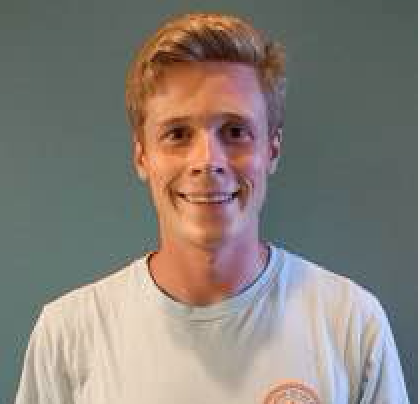
\includegraphics[width=1in,height=1.25in,clip,keepaspectratio]{josh.png}}]{Josh Kay}
is a graduate student researcher at the University of California, Berkeley. He is pursuing a Ph.D. under the direction of Professor Berhnard Boser. He received his Bachelor of Science degree in Electrical Engineering from the University of California, Santa Barbara in 2014.
\end{IEEEbiography}

\begin{IEEEbiography}[{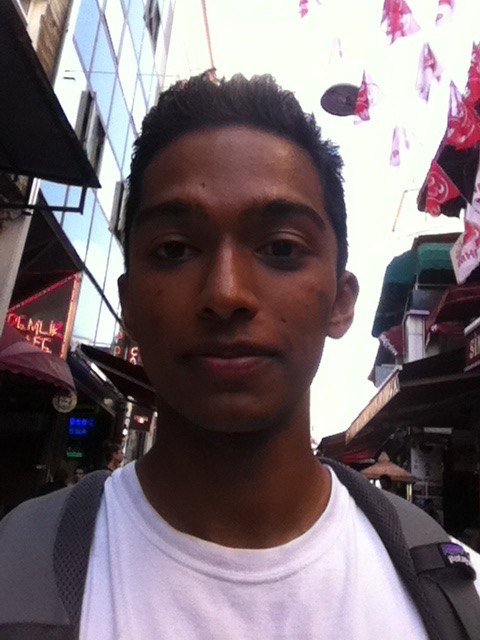
\includegraphics[width=1in,height=1.25in,clip,keepaspectratio]{karthik.jpg}}]{Karthik Gopalan}
is a graduate student researcher at the University of California, Berkeley. He is pursuing a Ph.D. under the direction of Professor Vladimir Stojanovi\'{c}. He received two Bachelor of Science degrees in Physics and Computer Science from the University of Maryland, College Park in 2015.
\end{IEEEbiography}

\end{document}


